\section{Results}
\label{sec:results}


Videos of all sixty run champions (pictured in Figs. \ref{fig:none}, \ref{fig:stress}, \ref{fig:pressure}) can be seen at
\href{https://www.youtube.com/playlist?list=PL7qssg0uLKTaFhaCRC0WviaGeOitOE8MR}{\textcolor{blue}{\textbf{\texttt{goo.gl/T5wZNQ}}}}.


\subsection{Evolvability.}

We first investigated whether environment-mediated morphological development affected evolvability (Fig. \ref{fig:run_champs}A).
At the termination of an evolutionary trial, we only consider the most fit individual{\textemdash}the run champion{\textemdash}from each of the twenty independent trials (Figs. \ref{fig:none}, \ref{fig:stress}, \ref{fig:pressure}).
After correcting for three comparisons, there was not enough evidence to reject the null hypothesis{\textemdash}that there is no difference between adaptive and nonadaptive robots, in terms of mean displacement{\textemdash}at the 0.05 level.

These results could be taken to suggest one of the following. 
Either the search space is sufficiently smooth prior to development (actuation and support are not as antagonistic as envisaged), or the proposed developmental mechanism is an insufficient smoothing 
mechanism
(successful ways to change stiffness as a linear function of stimuli are sparse in the search space).


\begin{figure}%[H]
\centering
{\Large \textbf{Non-developmental champions (Eq. \ref{eq:none})}}
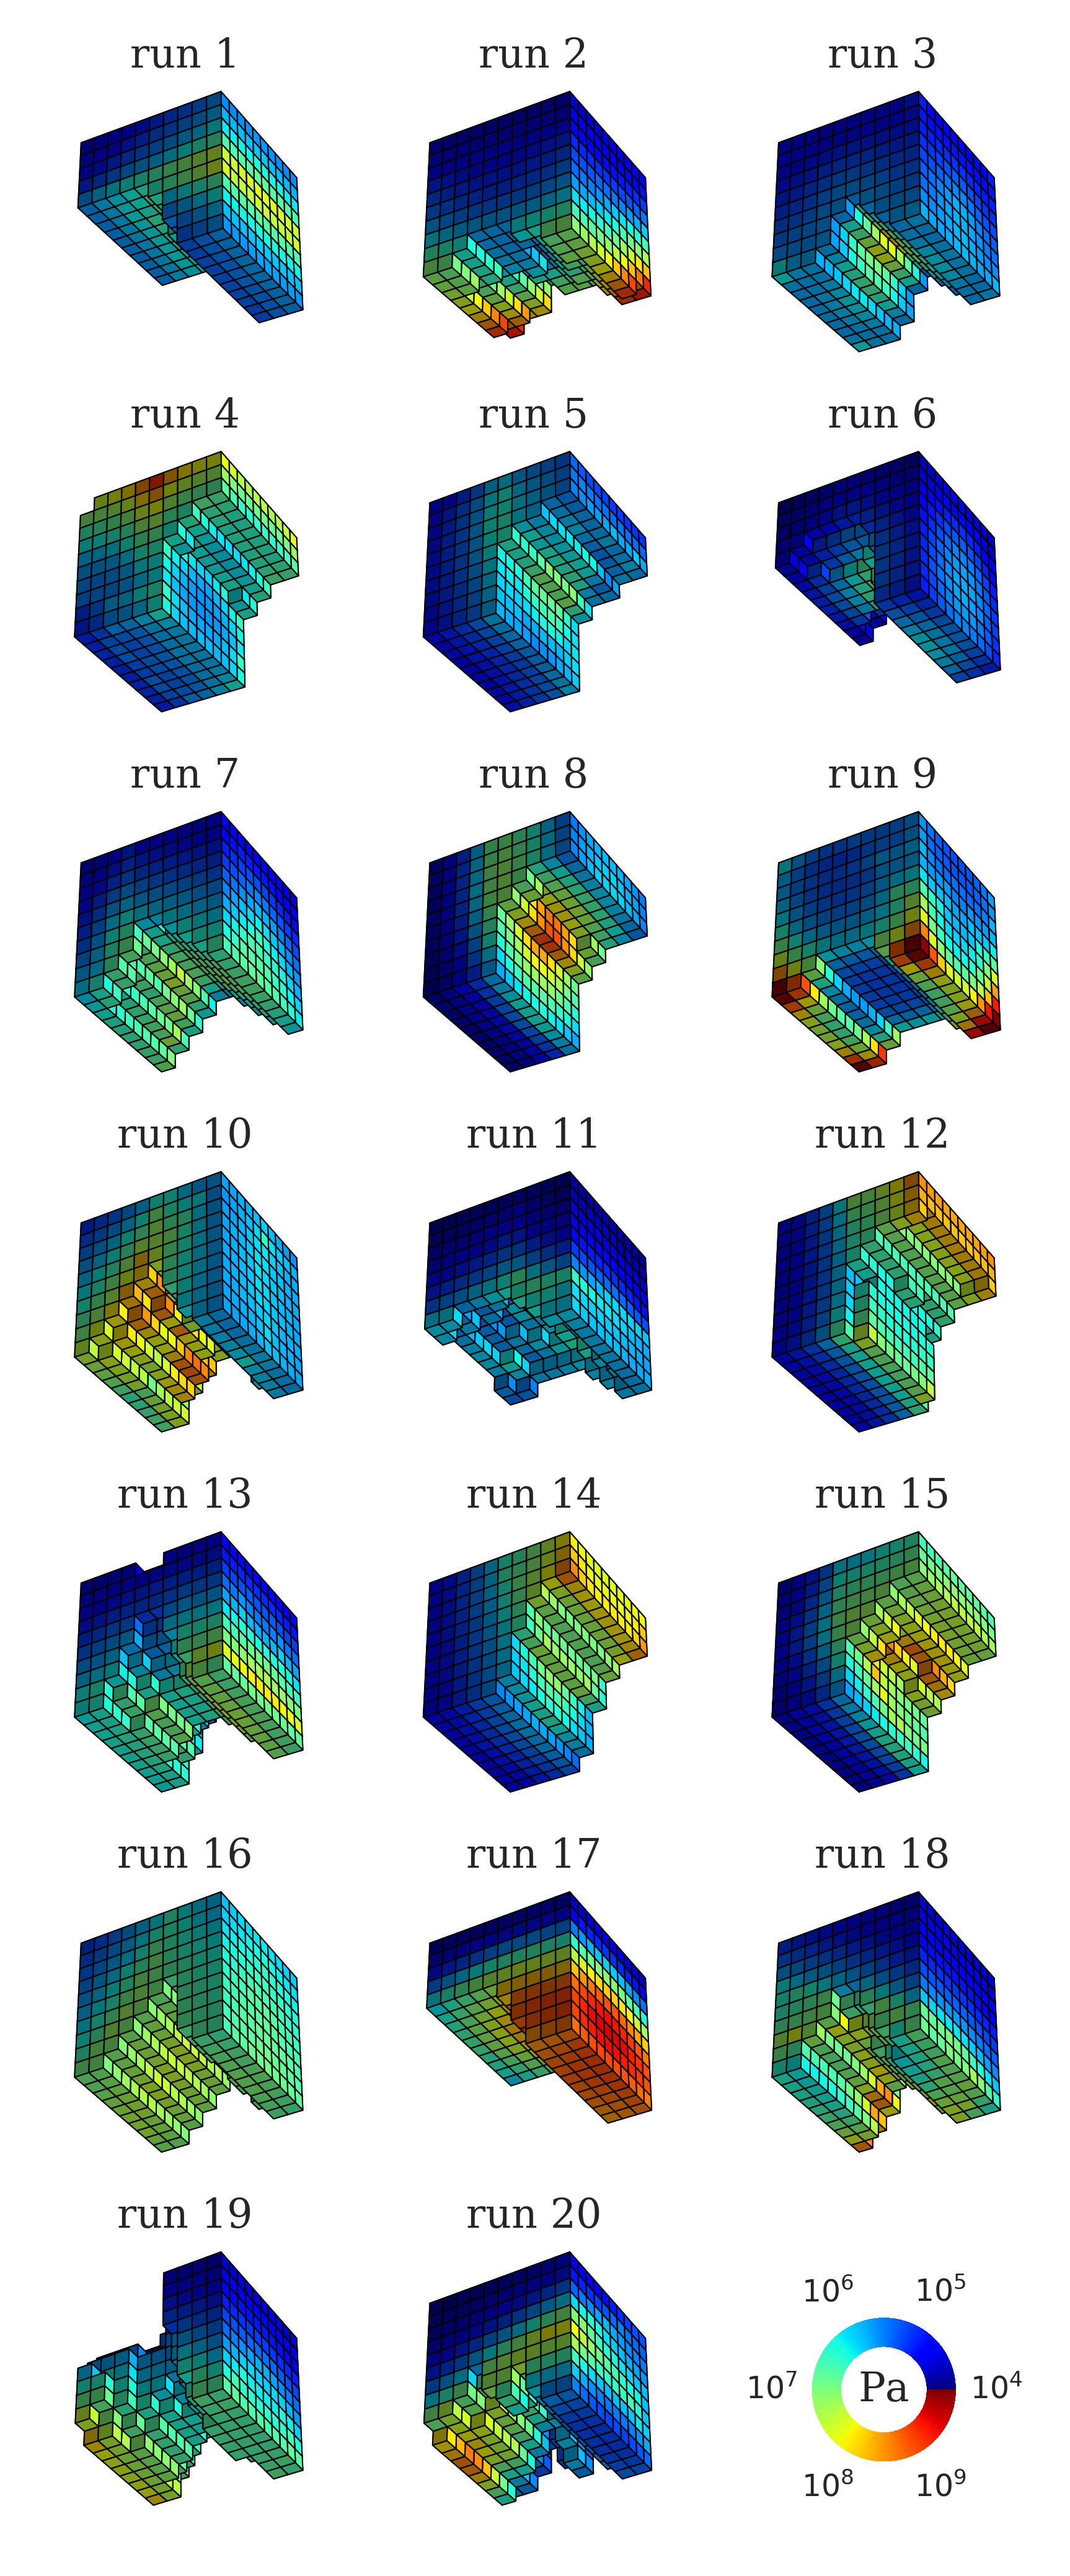
\includegraphics[width=0.5\linewidth]{Chapter06/img/zero_run_champs}
% \vspace{-2.5em}
\caption{\label{fig:none} Run champions colored by congenital stiffness, which ranges from 10\textsuperscript{4} to 10\textsuperscript{10} Pa. After settling under gravity, robots move toward the right-hand side of the page.}
\end{figure}


\begin{figure}%[H]
\centering
{\Large \textbf{Stress-adaptive champions (Eq. \ref{eq:stress})}}
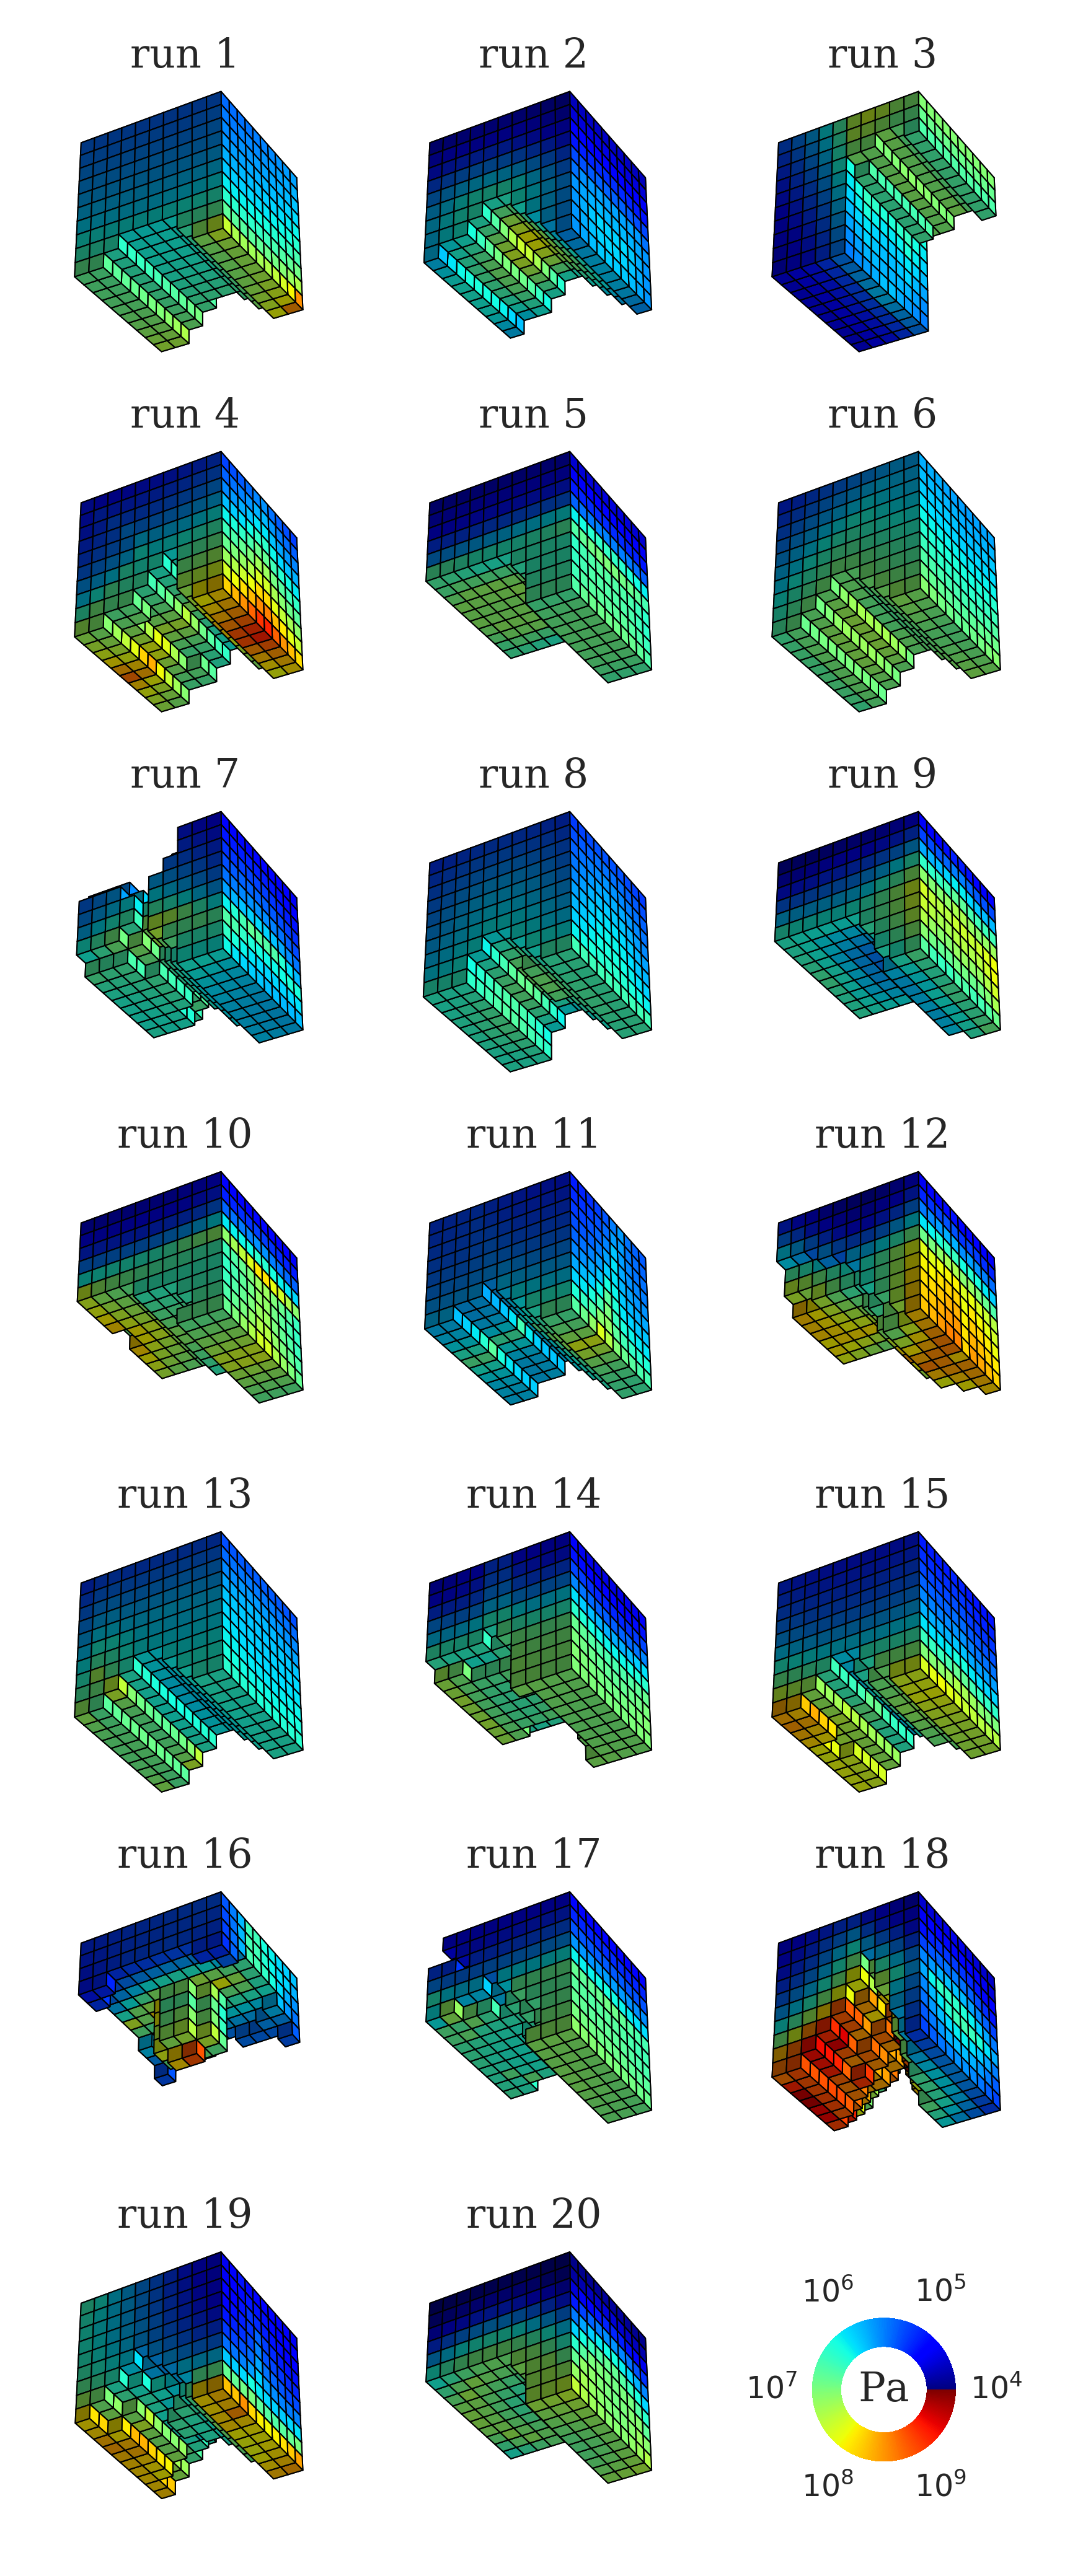
\includegraphics[width=0.5\linewidth]{Chapter06/img/stress_run_champs}
% \vspace{-2.5em}
\caption{\label{fig:stress} Run champions colored by congenital stiffness which can change during operation (ontogeny) in response to \textit{engineering stress.}}
\end{figure}

\begin{figure}%[H]
\centering
{\Large \textbf{Pressure-adaptive champions (Eq. \ref{eq:pressure})}}
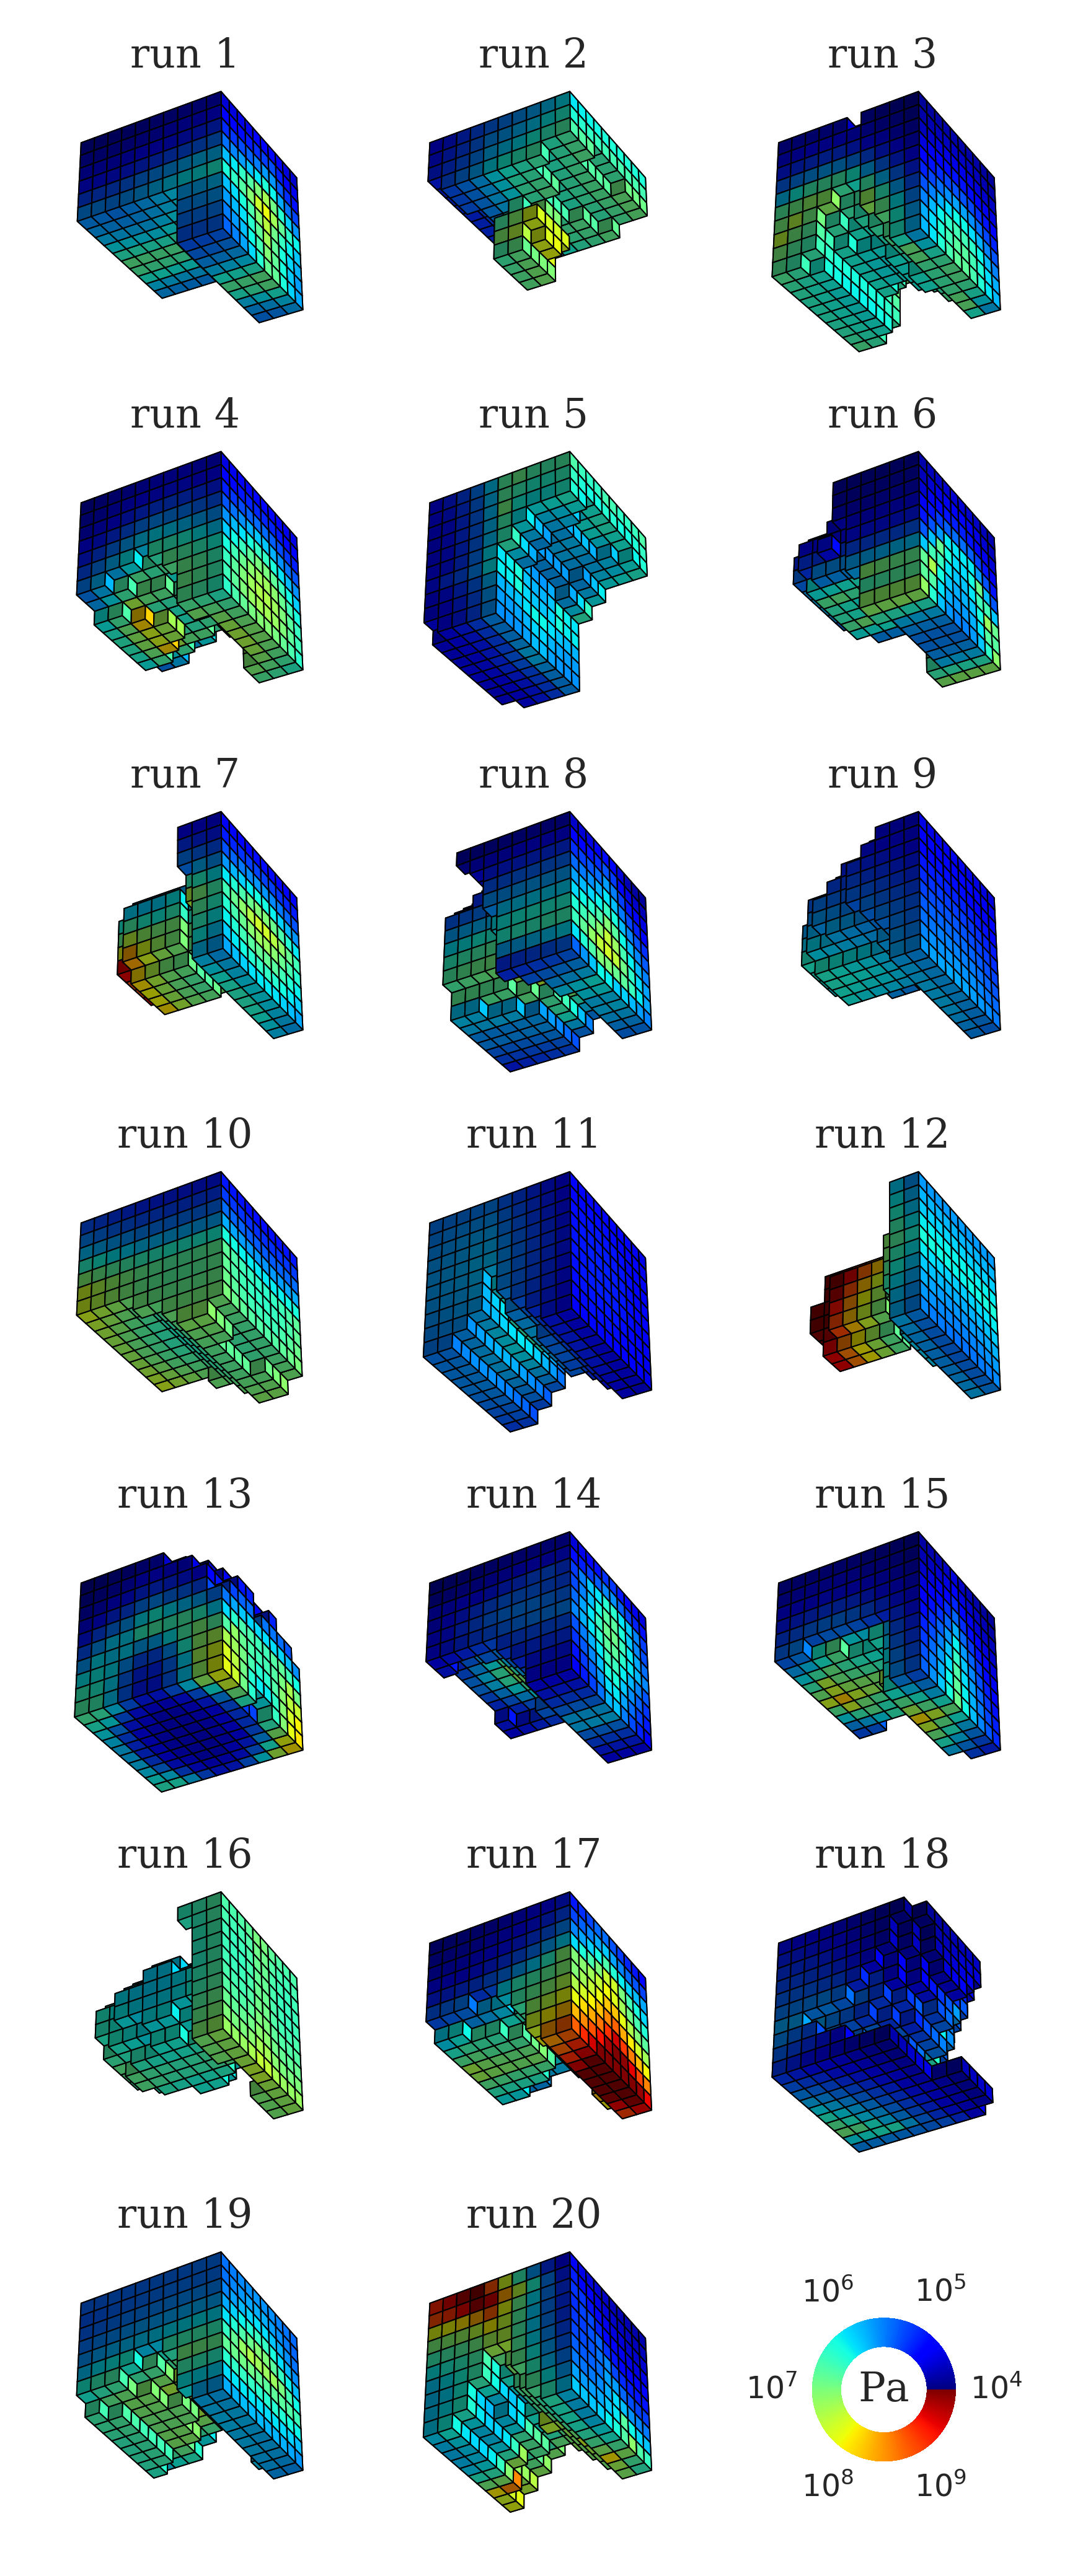
\includegraphics[width=0.5\linewidth]{Chapter06/img/pressure_run_champs}
% \vspace{-2.5em}
\caption{\label{fig:pressure} Run champions are colored by congenital stiffness which can change during operation (ontogeny) in response to \textit{pressure.}}
\end{figure}


\begin{figure*}[t]
\centering 
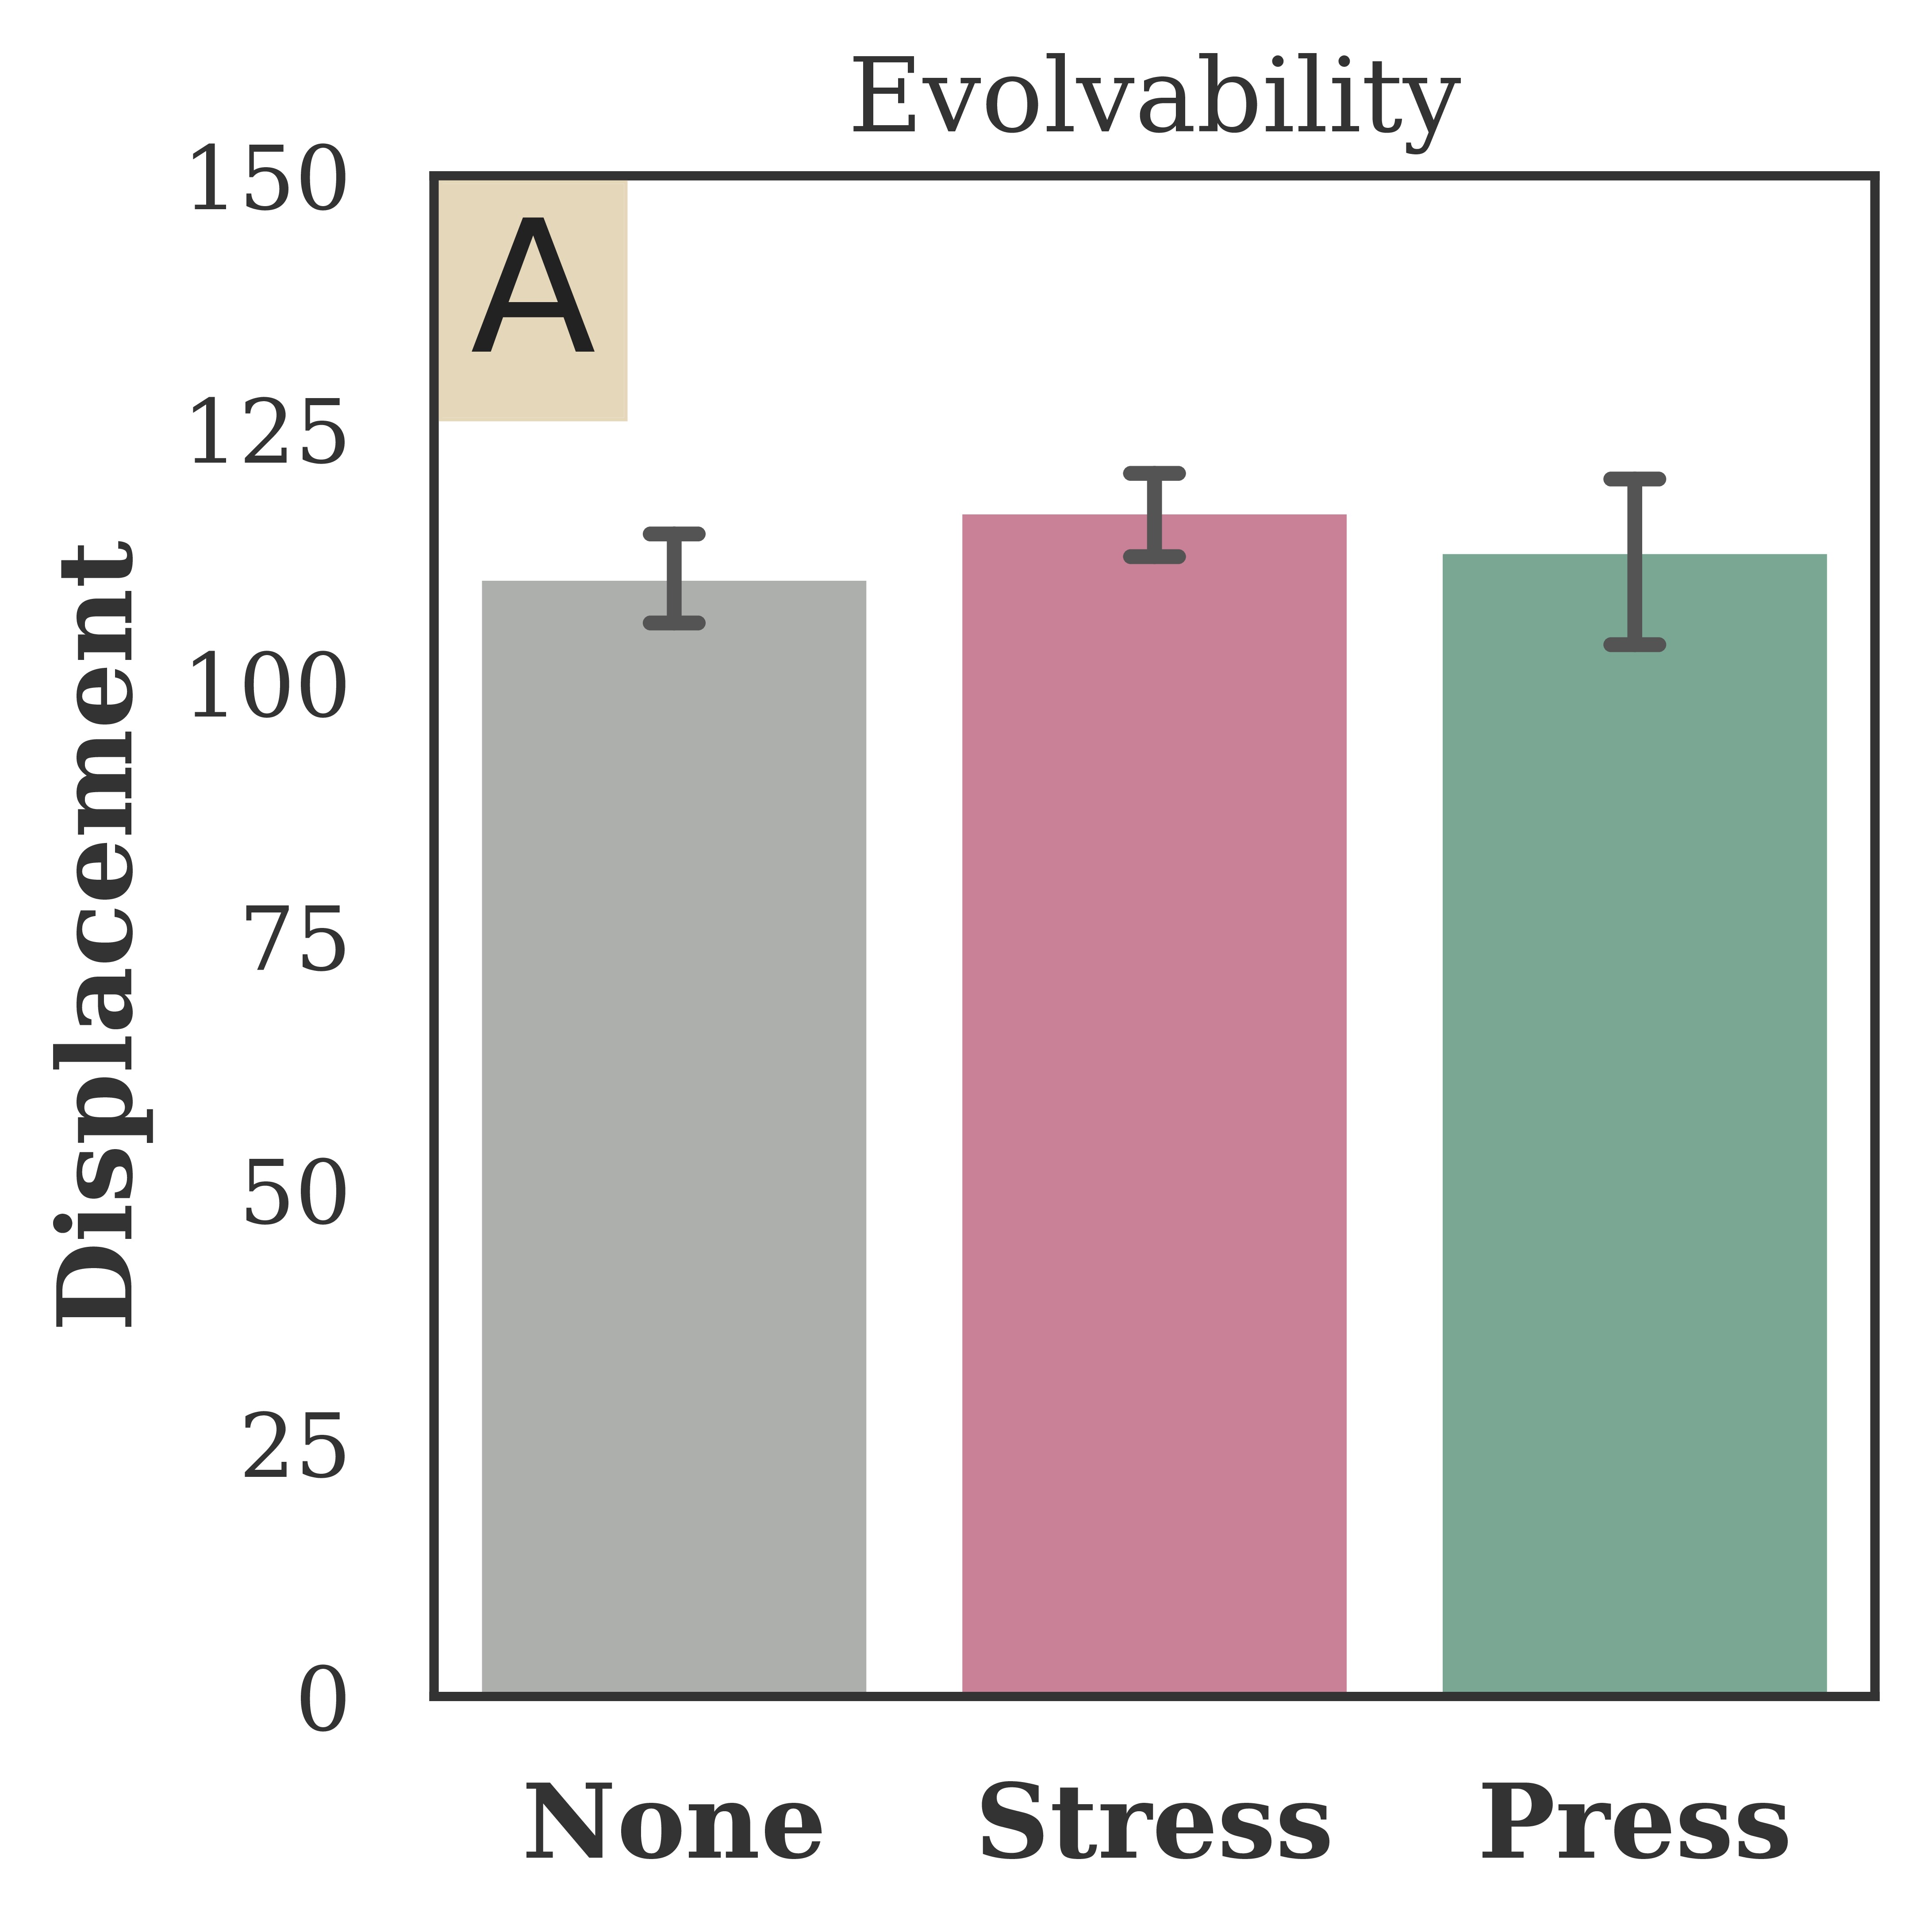
\includegraphics[width=0.32\linewidth]{Chapter06/img/Evolvability}
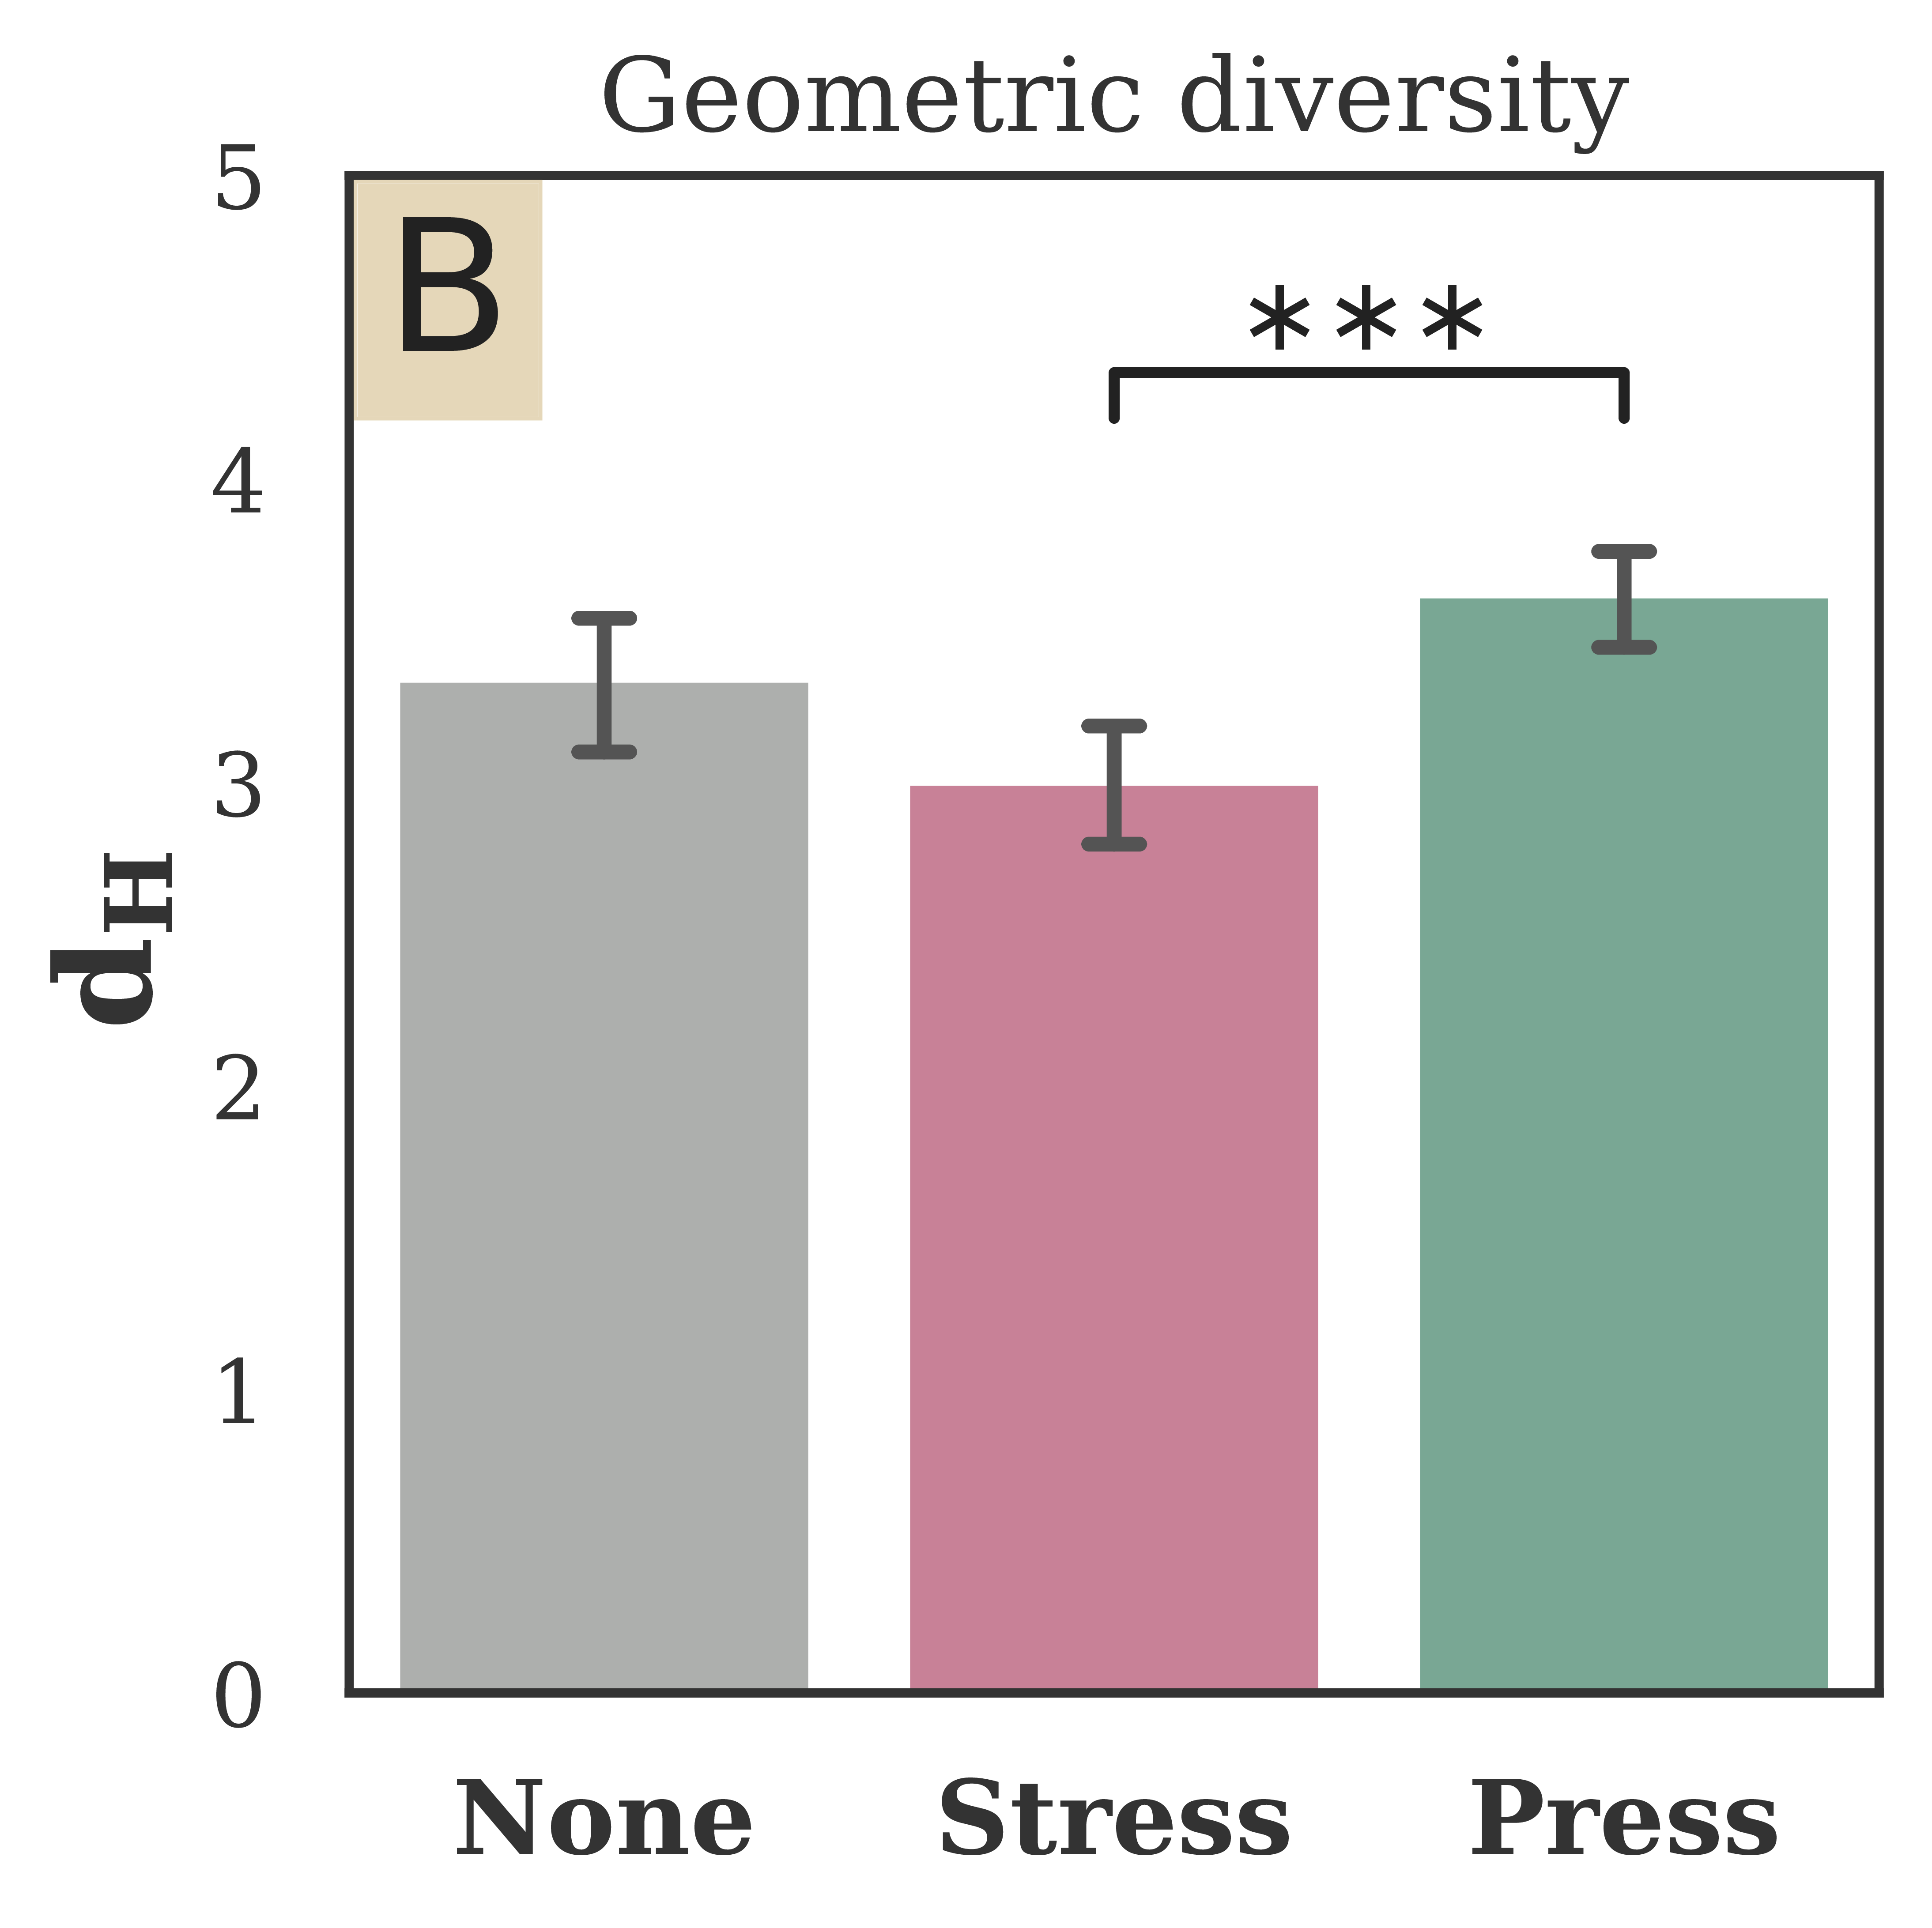
\includegraphics[width=0.32\linewidth]{Chapter06/img/Hausdorff} 
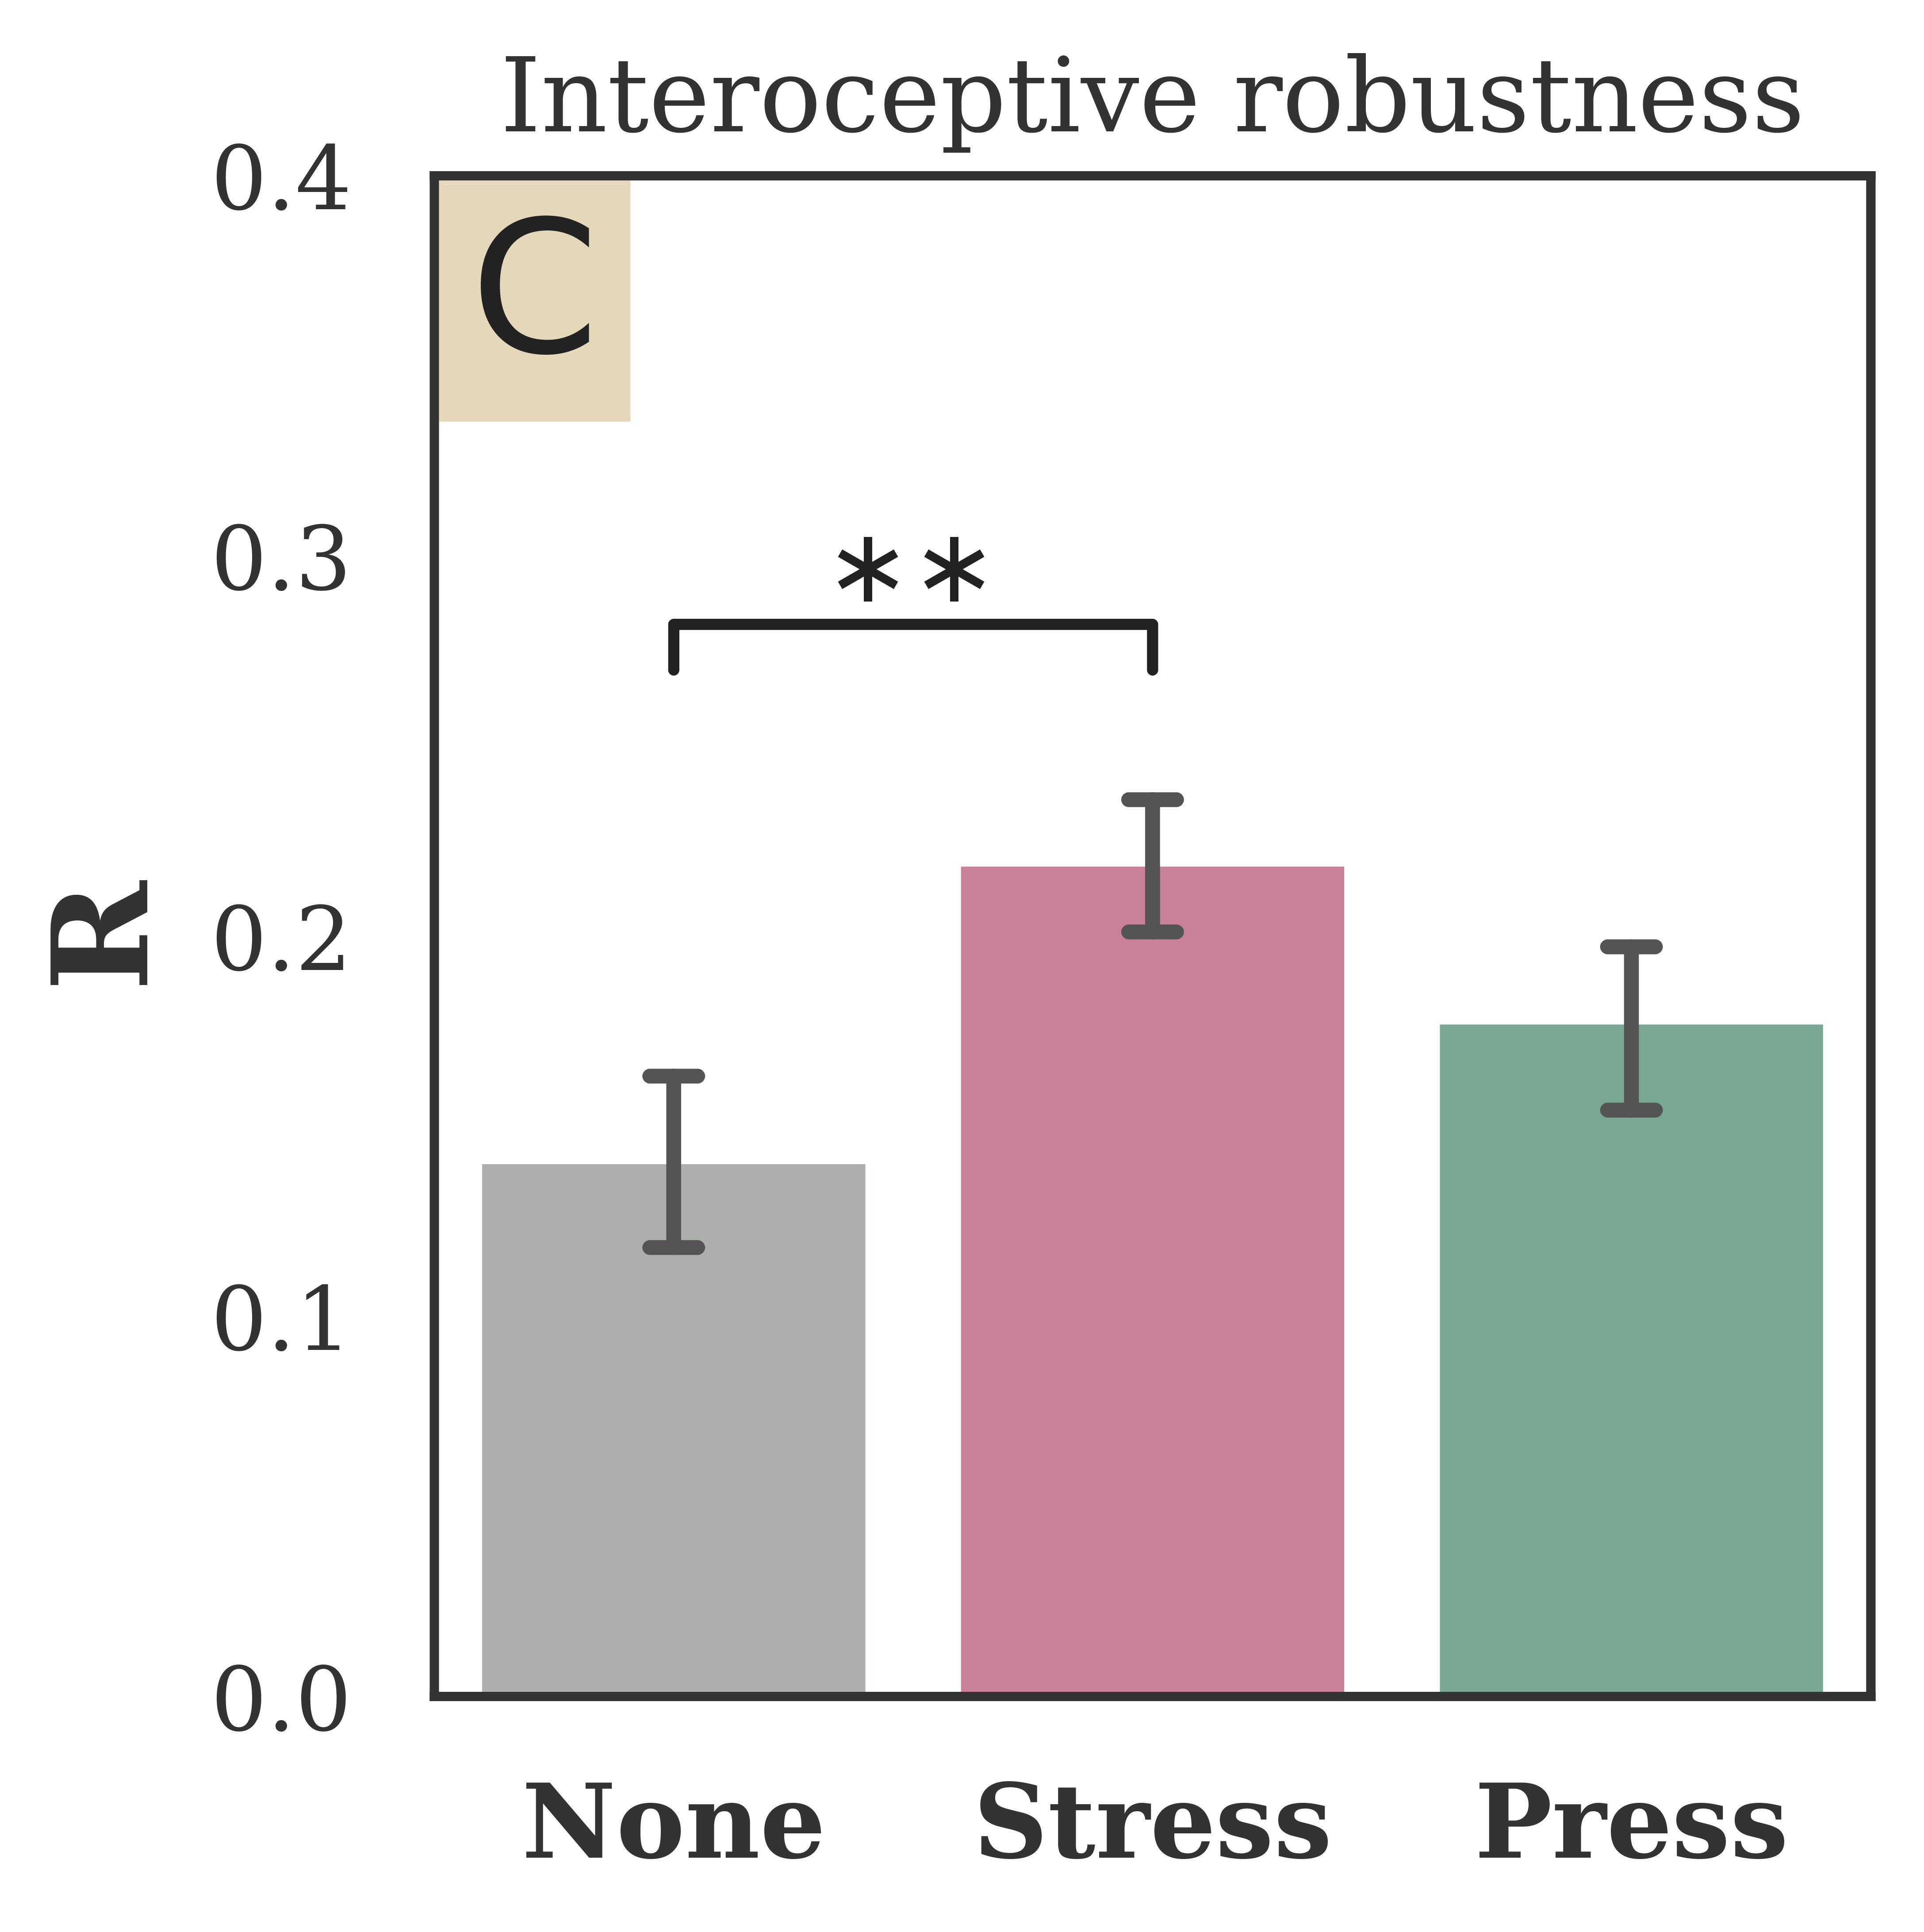
\includegraphics[width=0.32\linewidth]{Chapter06/img/Robustness}
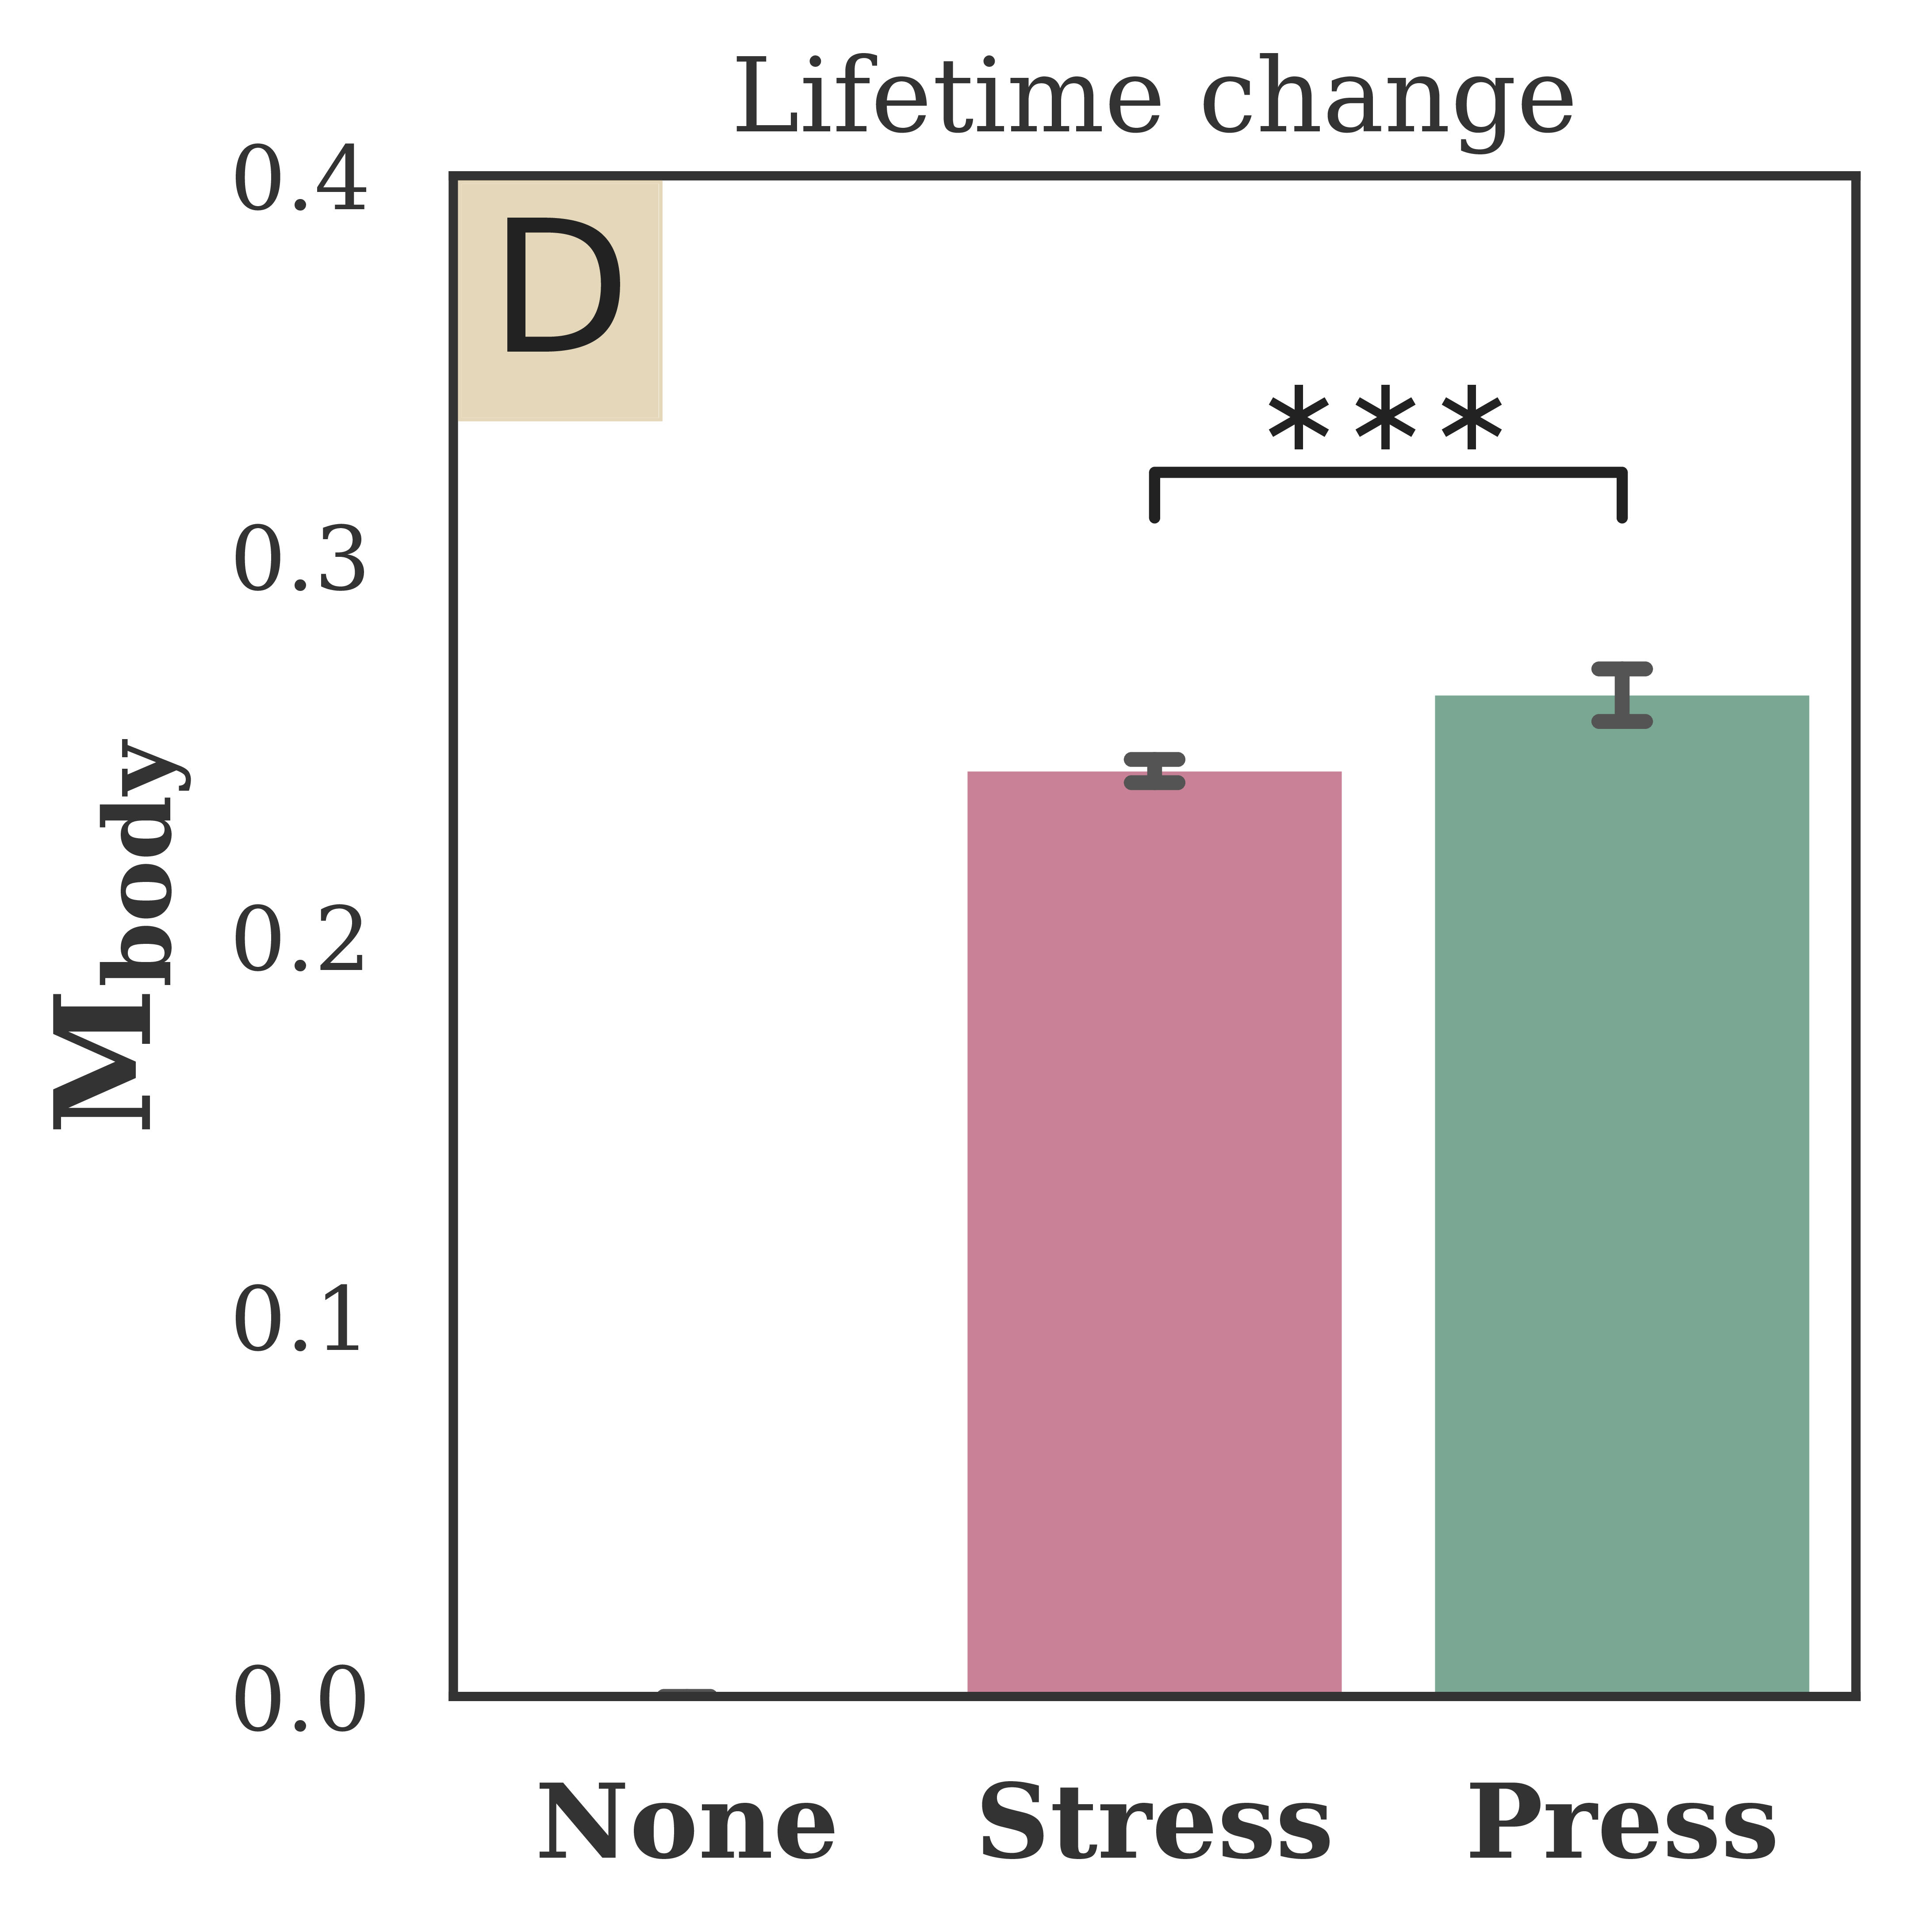
\includegraphics[width=0.32\linewidth]{Chapter06/img/Mean_Change}
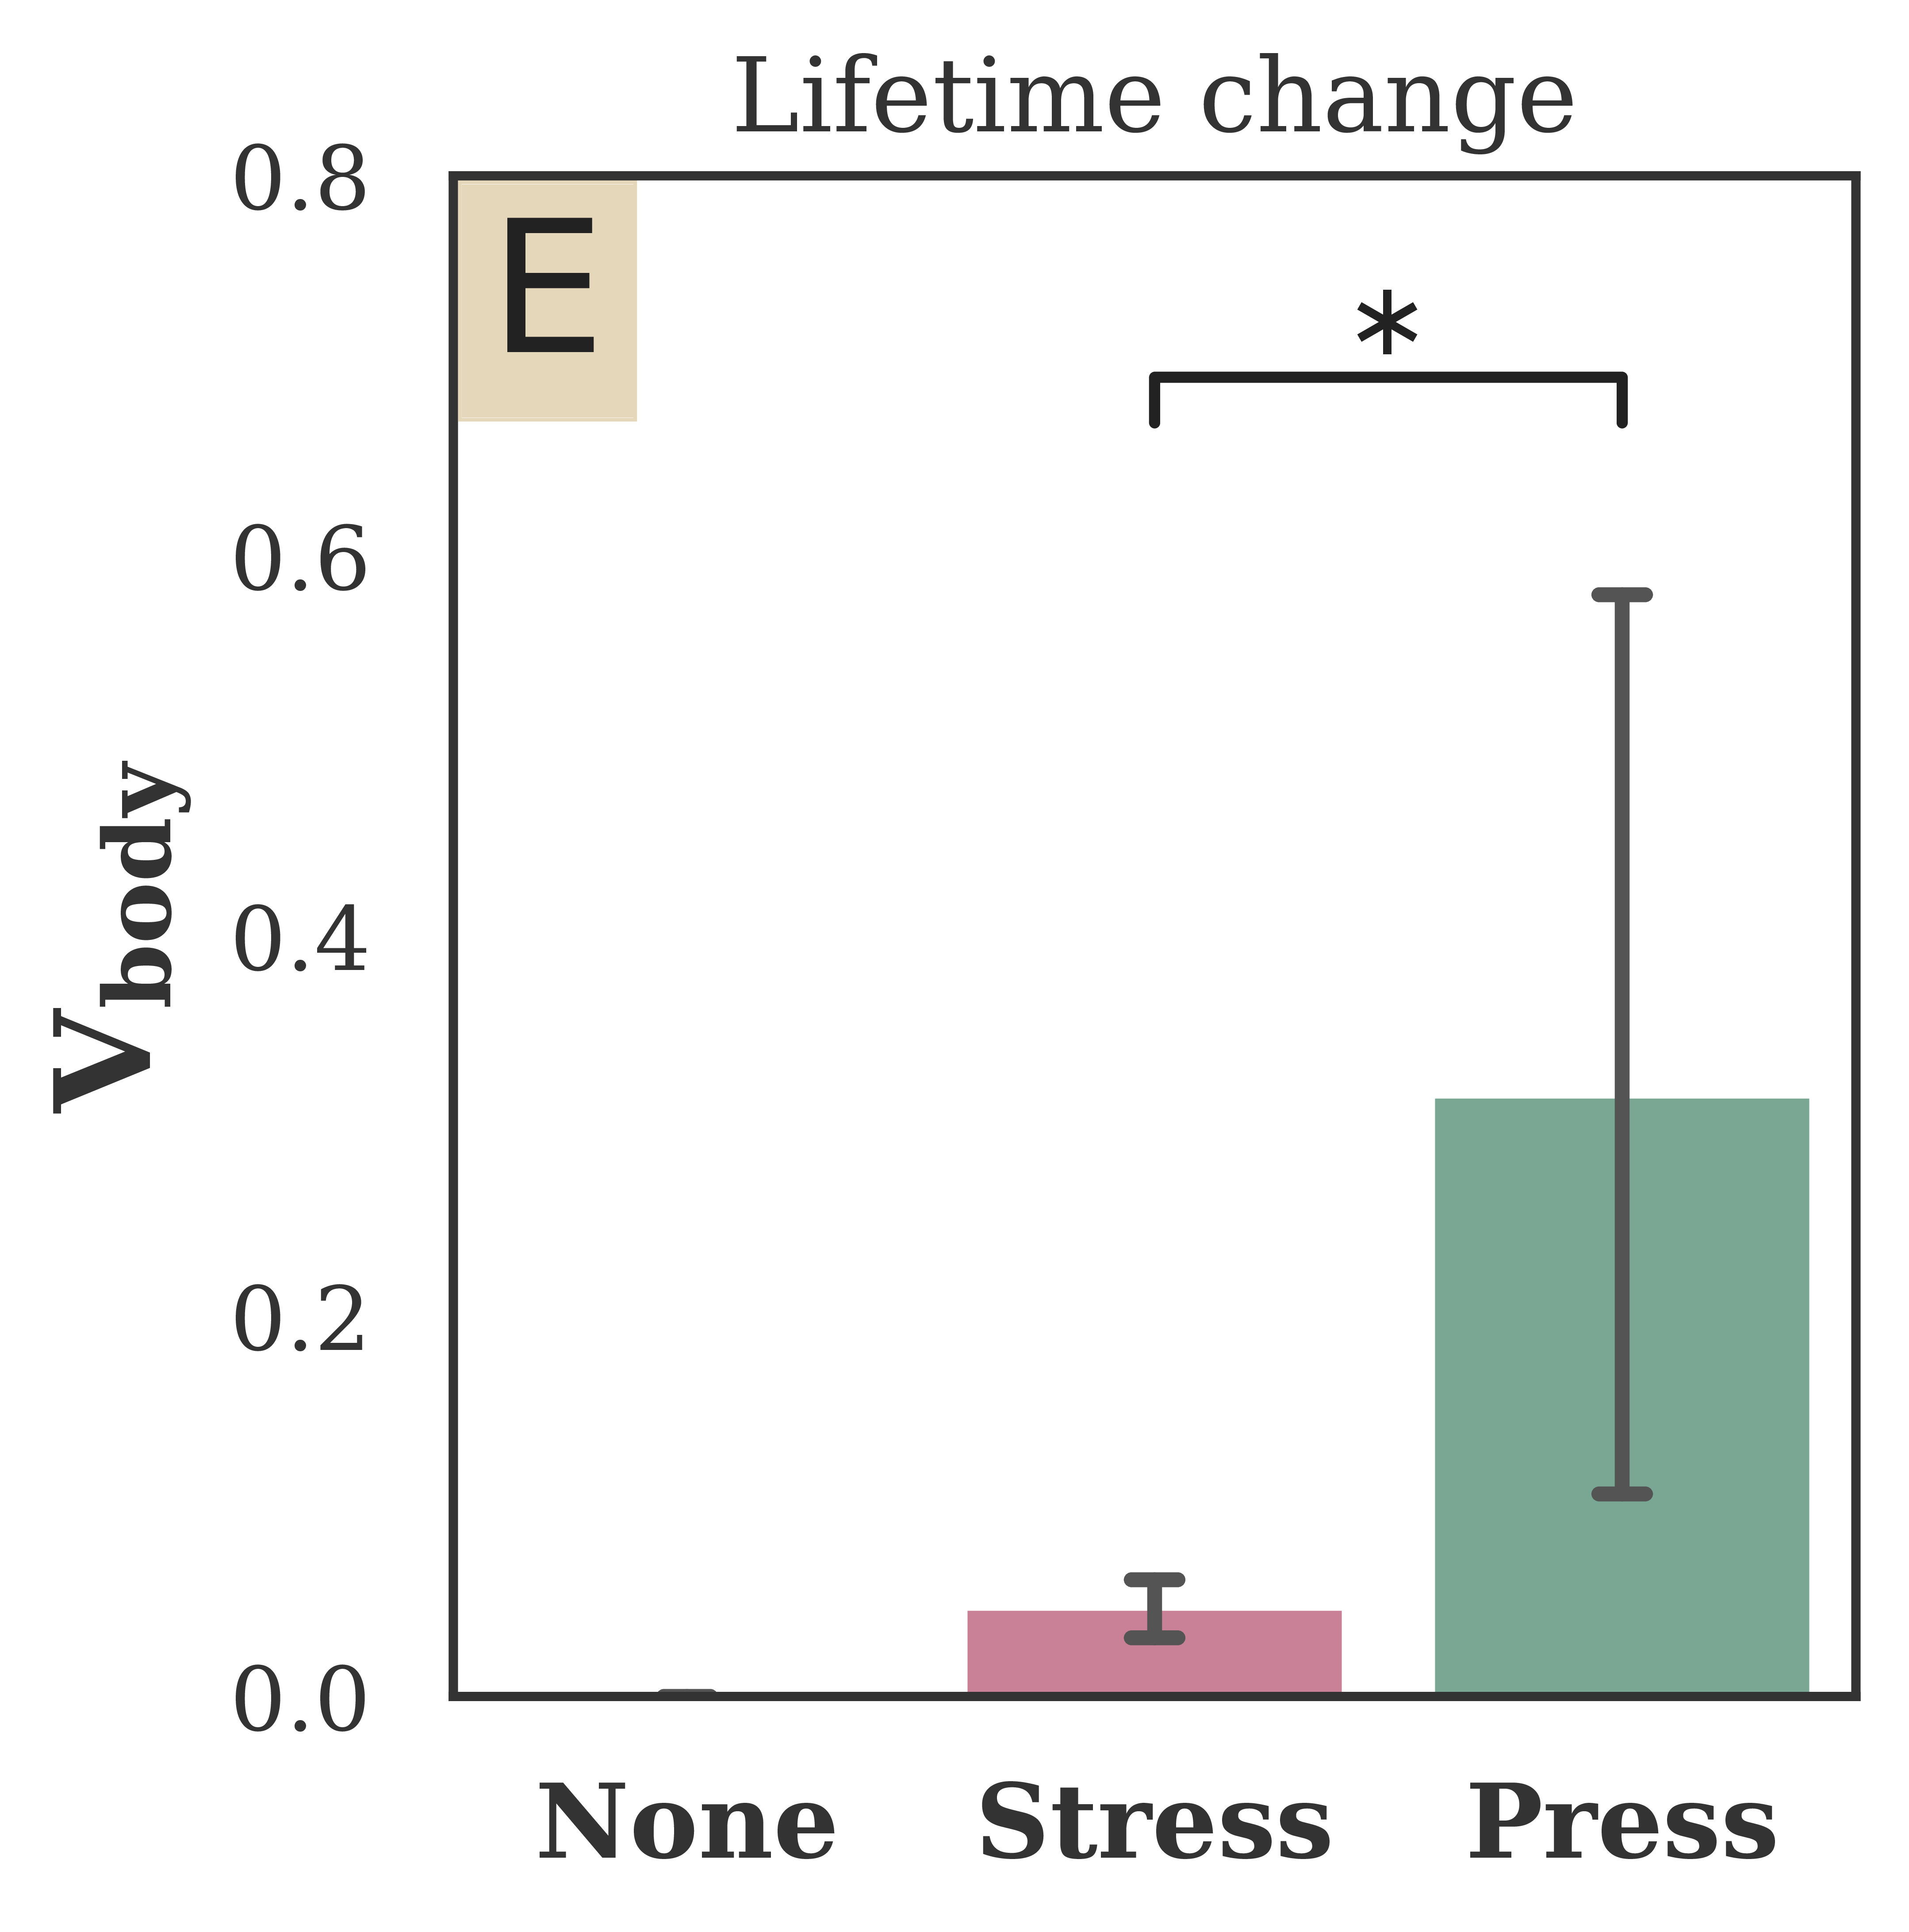
\includegraphics[width=0.32\linewidth]{Chapter06/img/Variance_Change}
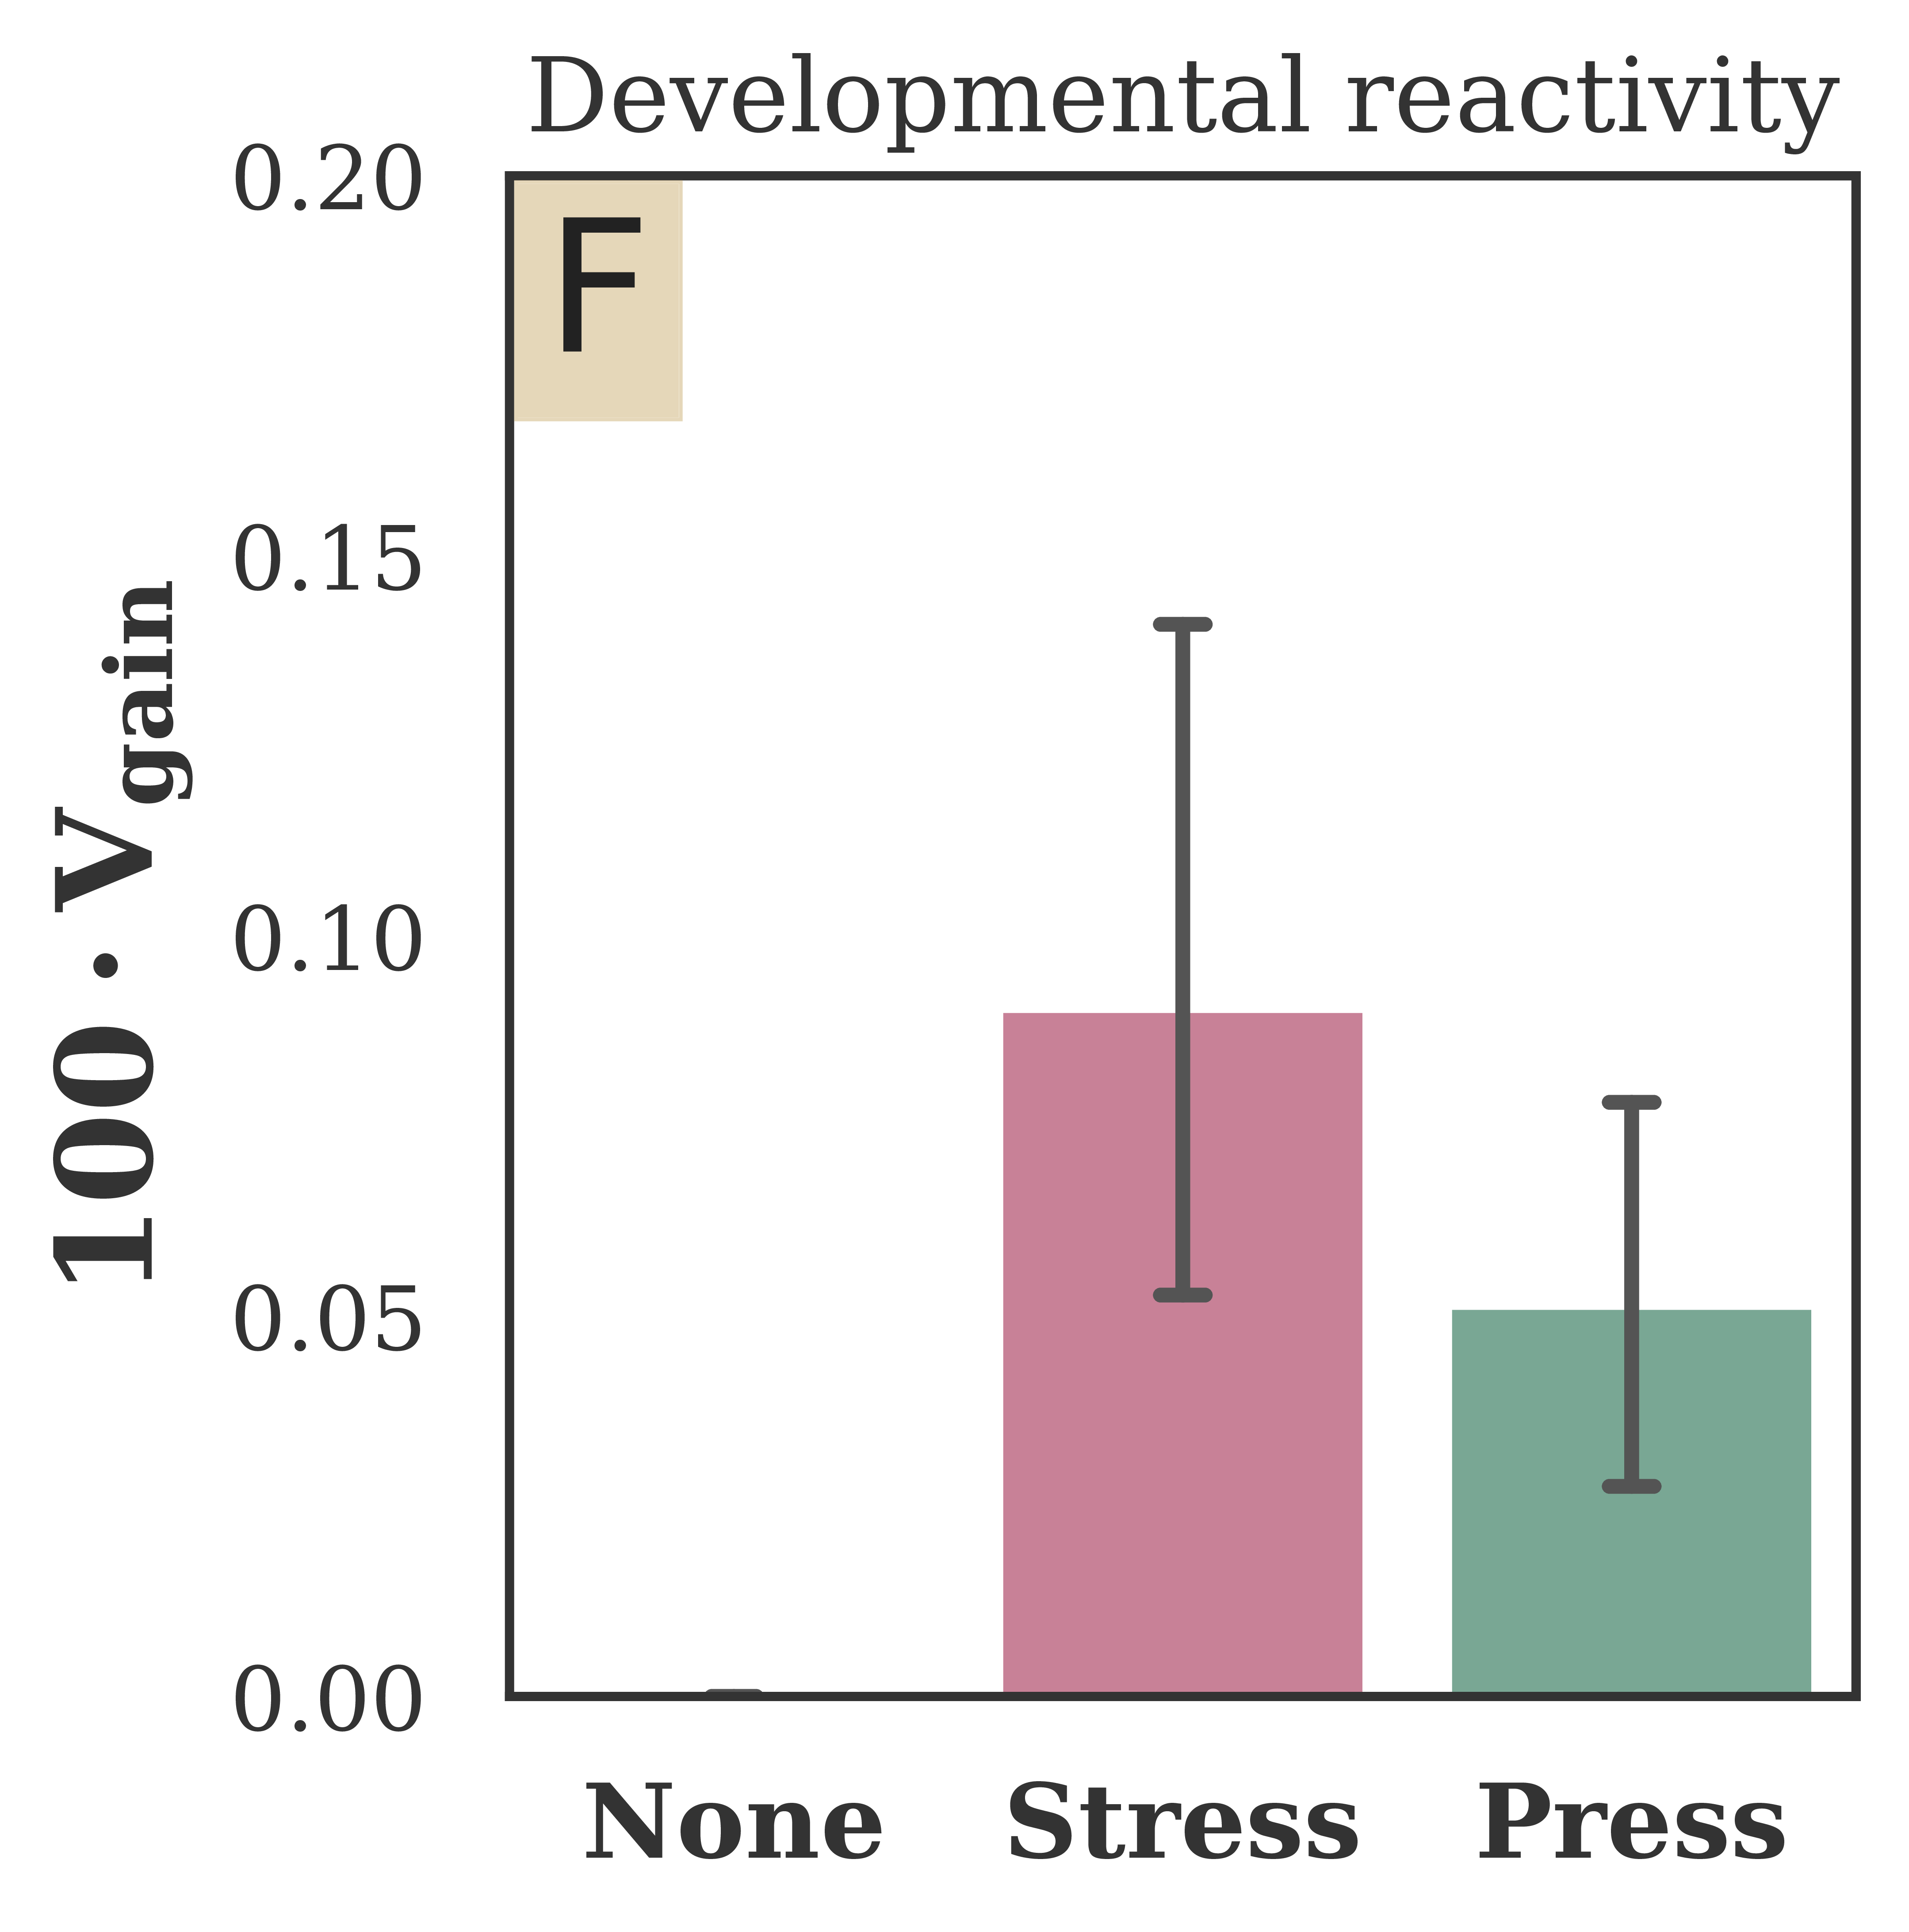
\includegraphics[width=0.32\linewidth]{Chapter06/img/Var_devo_gain}
\caption{\label{fig:run_champs} 
Means (with 95\% C.I.) for various statistics of the run champions, at generation 5000: 
(A) Fitness as the final displacement of a robot, measured by voxel-length units; 
(B) Diversity as the pairwise Hausdorff distances of robot geometries; 
(C) Robustness as the relative fitness (testing fitness divided by training fitness) after development is removed and a random stiffness distribution is introduced
into the champion's body (Eq. \ref{eq:robustness});
(D) Mean, taken across the body, of relative lifetime change in stiffness, as a measure of the lack of canalization (Eq. \ref{eq:mu}; lower bars indicate more canalization);
(E) Variance, taken across the body, of relative lifetime change in stiffness, as a measure of heterogeneity/nonuniformity in developmental reactions (Eq. \ref{eq:sigma});
(F) Variance, taken across the body, of the coefficients/gain of developmental reactivity (Eq. \ref{eq:sigma-gain}).
}
\end{figure*}


\subsection{Geometric diversity.}

We investigate morphological diversity next by
employing the Hausdorff distance $d_H$ as a metric to compare the similarity of two robot geometries, $A$ and $B$.
For each voxel in $A$, the closest voxel in $B$ is identified, according to euclidean distance $d$.
Similarly, for each voxel in $B$, the closest voxel in $A$ is identified.
The Hausdorff metric is the larger of these two distances. 
Formally,
\begin{equation}
\label{eq:hausdorff}
d_H(A,B) = \max\{\,\sup_{a \in A} \inf_{b \in B} d(a,b),\; \sup_{b \in B} \inf_{a \in A} d(a,b)\,\} \, . %\mbox{.}
\end{equation}
Informally, two robots are close in the Hausdorff distance if every voxel of either robot is close to some voxel of the other robot. 
 

We calculated the Hausdorff distance between each of the $\binom{20}{2}=190$ possible pairings of the 20 run champions (Fig. \ref{fig:run_champs}B).
Because $d_H(A,B)$ depends on the orientations of $A$ and $B$, we rotate $B$ in the $xy$ plane (0, 90, 180, and 270 degrees) and the $yz$ plane (0 and 90 degrees), and select the rotation that creates the smallest $d_H(A,B)$.

We found the evolved body shapes of pressure-adaptive robots to be more diverse than those of stress-adaptive robots $(P<0.001)$.
We did not find a significant difference, at the 0.05 level, between adaptive and nonadaptive treatments using this particular measure of morphological diversity.

Across all three treatments,
there appear on visual inspection to be three types of geometries (Figs. \ref{fig:none}-\ref{fig:pressure}): a $\Pi$ robot with wide posterior and anterior legs; a $\Gamma$ robot whose legs meet perpendicularly; and a $\Upsilon$ robot that connects a (mainly cylindrical) leg perpendicularly to the center of a $10\times10$ vertical plane.
Depending on how one counts, the $\Upsilon$ species can be seen in at most one nonadaptive robot (Fig. \ref{fig:none}, run 19), two stress-adaptive robots (Fig. \ref{fig:stress}, runs 7 and 16), and six pressure-adaptive robots (Fig. \ref{fig:pressure}, runs 2, 6, 7, 9, 12, and 16).
Pressure-adaptive robots have more diversity by virtue of more $\Upsilon$ robots.


\subsection{Interoceptive robustness.}

To investigate the relative robustness (if any) across the three treatments,
in the following experiment, development was manually removed from the stress- and pressure-adaptive run champions.
We then tested the sensitivity of the resulting reduced robots to their evolved congenital stiffness distribution (Fig. \ref{fig:run_champs}C).
To do so, we replaced the evolved network dictating material stiffness, $\mathbb{C}_2,$ with a random number generator that draws from the same range of possible stiffness ($10^4 - 10^{10}$ Pa).
That is to say, we `built' the evolved run champions without any errors in the specifications of geometry and actuation, but completely ignored the evolved specifications of their material stiffness, replacing them instead with random noise.
We then calculated the relative fitness
\begin{equation}
\label{eq:robustness}
R = F_{\text{test}}\,/\,F_{\text{train}} \, ,
\end{equation}
where $F_{\text{train}}$ is the fitness achieved using the evolved stiffness and $F_{\text{test}}$ is the fitness when tested with a random stiffness distribution.
We repeated this process ten times for each run champion, each time drawing a new random stiffness distribution.


We found that, compared to nonadaptive robots, reduced stress-adaptive robots 
were 
% are
more robust to this (extreme) discrepancy between training and testing stiffness distributions $(P < 0.01)$.
These results are consistent with the 
found correlation between development and robustness
\cite{miller2004evolving,bongard2011morphological,kriegman2017morphological}.
However, the results here indicate that this correlation is contingent on the kind of environmental
signal the developing agent responds to: there was no difference between pressure-adaptive and nonadaptive robots in this regard, at the 0.05 level.

This implies that by behaving interoceptively with respect to engineering stress, robots evolved the ability to ameliorate large deviations from their expected material properties, but by behaving interoceptively with respect to pressure, robots did not evolve this character.
Because development was manually removed beforehand, robustness in our case was not a matter of changing one's body, as in the example of plant growth \citep{sultan2000phenotypic}; rather, it is an intrinsic property of structure (geometries and actuation patterns) educed from ancestors who changed in response to one particular internal state (stress), but not from those who responded to another (pressure).


The difference in robustness between nonadaptive robots and stress-adaptive, but not pressure-adaptive robots, could be due in part to the fact that there are simply more pressure-adaptive $\Upsilon$ robots than stress-adaptive $\Upsilon$ robots.
While $\Upsilon$ robots tend to be more fit than $\Pi$ and $\Gamma$ robots $(P_{\Pi}<0.05;\, P_{\Gamma}<0.05)$,
they also appear to exploit their material properties to a greater degree, and are thus more sensitive to changes in its constitution, compared to $\Pi$ and $\Gamma$ robots $(P_{\Pi}<0.05;\, P_{\Gamma}<0.01)$.

The $\Upsilon$ robot generates movement by pushing off its posterior leg,
which must be rigid enough to support itself as well as 
propel forward the center portion of its anterior wall 
(e.g.~run 12 in Fig.~\ref{fig:pressure}).
The robot loses kinetic energy, which is stored as elastic strain energy in the spring-like voxels between the wall's center and edge.
The most strain is present in the dorsal portion of the anterior wall.
The springs recoil, restoring kinetic energy and generating forward motion.
If the posterior leg is too soft, or the dorsal anterior wall too rigid, the $\Upsilon$ robot can suffer a large drop in performance.

Differences in geometry, however, shed no light on why (the reduced) stress-adaptive robots are more robust than nonadaptive robots:
the level of significance $(P<0.01)$ does not change after removing the only nonadaptive robot that could possibly be classified as $\Upsilon$ (Fig. \ref{fig:none}, run 19). 
Thus we continue our investigation by analyzing how stress and pressure might differentially affect the rate of developmental reactions.


\subsection{Canalization.}

% According to Waddington \citep{waddington1942canalization}, 
% \begin{quote}
% developmental reactions \textit{as they occur in organisms submitted to natural selection}, are in general canalized. That is to say, they are adjusted so as to bring about one definite end-result regardless of minor variations in conditions during the course of the reaction.
% \end{quote}
One indication of canalization \citep{waddington1942canalization,kriegman2017morphological} in our system is given by the magnitude of $\alpha_i$ in each voxel, as defined by Eqs. \ref{eq:stress} and \ref{eq:pressure}.
However, this is but one of two necessary ingredients for a developmental reaction: it indicates bodywide responsiveness to \textit{potential} stimuli, but ignores the \textit{actual} stimulus.

Thus, as proxy for canalization, we measured the amount of morphological change in reaction to local stimulus, during evaluation.
More precisely, we recorded the mean, across the body, of relative lifetime change in stiffness
\begin{equation}
\label{eq:mu}
M_{\text{body}} = \frac{1}{\#\gamma} \sum_{i \in \gamma} \left| k_i^{+}/k_i^{\circ}-1 \right| ,
\end{equation}
where 
$k_i^{\circ}$ 
is the congenital stiffness,
$k_i^{+}$ is the final stiffness, and
$\gamma = \{i : g_i = 1 \}$ contains the coordinates $i$ of each voxel $g_i$ present in the (bit array) geometry which has cardinality $\#\gamma$ (total voxels). 
Less change---lower $M_{\text{body}}$---indicates more canalization.

On average, voxels in stress-adaptive robots change their relative stiffness less than voxels in pressure-adaptive robots $(P<0.001)$ (Fig. \ref{fig:run_champs}D).
In other words, developmental reactions are canalized to a greater extent in stress-adaptive robots.
It follows, then, that the treatment with increased robustness was also the treatment with increased canalization.

To get a sense of the consistency of developmental reactions, as they occur \textit{across the body} of evolved robots, we also recorded the spatial variance of this relative lifetime change 
\begin{equation}
\label{eq:sigma}
V_{\text{body}} = \text{Var}_{i \in \gamma} \left(\,\left| k_i^{+}/k_i^{\circ}-1 \right|\,\right) .
\end{equation}
By this measure, stress-adaptive robots exhibit more uniform reactions than pressure-adaptive robots $(P<0.05)$ (Fig. \ref{fig:run_champs}E).
% \textcolor{red}{This is interesting, but I don't really know what to make of it... do we have an interpretation of the possible implications or importance of the uniformity of a developmental process? (is this due to the more localized/acute forces of pressure/stress?)}

Taken together, then, we may say that the developmental reactions of stress-adaptive robots are more uniform in space 
(lower $V_{\text{body}}$; Fig. \ref{fig:run_champs}E), 
and more canalized in magnitude (lower $M_{\text{body}}$; 
Fig. \ref{fig:run_champs}D) than those of pressure-adaptive robots.
Pressure-adaptive robots therefore experience larger and more localized changes in stiffness during their lifetime.

There are two possibilities that could explain this more localized change in stiffness in the pressure-adaptive robots.
One possibility is that there is greater variance among the $\alpha_i$ in the pressure-adaptive robots.
The alternative is that there is greater variance in the application of pressure throughout the body.
% greater uniformity in reaction to stress than in reaction to pressure (Fig. \ref{fig:run_champs}D).
To test the first possibility, we first normalized $\alpha_i$ in pressure- and stress-adaptive robots
by the differing ranges of $\alpha$ that evolved in the pressure-adaptive (-5.36 to 5.63) 
and stress-adaptive (-10.00 to 6.42) robots.
Then we took the variance of $\alpha_i$ across the body of each run champion, individually:
\begin{equation}
\label{eq:sigma-gain}
V_{\text{gain}} = \text{Var}_{i \in \gamma} \tilde{\alpha_i} \,, \quad \text{where} \;\, \tilde{\alpha_i}=\frac{\alpha_i-\alpha_{\text{min}}}{\alpha_{\text{max}}-\alpha_{\text{min}}}  \,.
\end{equation}
We found no evidence to support the hypothesis that $\alpha_i$ in pressure-adaptive robots vary more (or less) in space than those in stress-adaptive robots (Fig. \ref{fig:run_champs}F).


Therefore, because there is no difference in the variation of $\alpha_i$ (Fig. \ref{fig:run_champs}F), and because  $\alpha_i$ cannot change during operation (Eqs. \ref{eq:stress} and \ref{eq:pressure}), it follows that pressure was generally much more localized within
the bodies of the pressure-adaptive robots than stress within the bodies of the stress-adaptive robots.
In other words, the entire body plan encountered stress, but only a small portion of the body encountered appreciable pressure.
(An example of this localized response to localized pressure can be seen in Fig. \ref{fig:calluses}.)
We hypothesize that this global spread of stress is the likely cause of increased robustness in the stress-adaptive robots
(Fig. \ref{fig:run_champs}C).

% \subsection*{Evolutionary history.}

% We tracked the ancestral lineages: a line of descent originating from a randomly created ancestor, which can be traced forward in a sequence of progeny, terminating with the respective run champion (Fig. \ref{fig:evo-hist}).






